\documentclass{article}
\usepackage{graphicx, float, url, hyperref, afterpage, amsthm, amsmath, multirow}
\title{Independent Component Analysis}
\author{Joshua Frankie Rayo\\2011-19612\\CS 280 Programming Assignment 4}
\date{\today}

\begin{document}

\maketitle
\tableofcontents

\section{Introduction}
	In this paper the independent component analysis was used to separate the source signals from a set of observations, assuming linear mixture and the sources are statistically independent. Five sound observations are the input data and ICA algorithm outputs the five independent sound sources. Several factors were taken into account relevant to the algorithm: input sampling rate, centering, whitening and appropriate contrastive function. Finally, the residual was used to measure the reconstruction performance of the algorithm.
\section{Methodology}
The code is made using Python, a high level, general-purpose programming language that is relatively easy to learn and has very good features in list manipulation. The \texttt{sklearn} library of Python was used to execute the FastICA algorithm. Other libraries used are \texttt{numpy} and \texttt{scipy}.

\subsection{Input Data}
The audio files \texttt{mic[1-5].wav} contains syncronized audio recordings captured by five microphones positioned at five different locations. Each sound file contains mixture of 5 independent signals with varying volumes. Each sound file was read using \texttt{scipy.io.wavfile.read()} that determines its sampling rate and wave sequence of length 191258. The sampling rate is 22050 Hz. The mixture matrix was formed by augmenting the wave sequences, which as of size 191258x5.

\subsection{Running the FastICA algorithm}
Different parameters are necessary to run the algorithm, listed below:
\begin{itemize}
	\item appropriate input sampling rate
	\item whether centering is required for preprocessing
	\item whether whitening is necessary for preprocessing
	\item appropriate contrastive function $G(y)$
\end{itemize}
these parameters are experimented to determine which produces the best unmixing of the sources.

There are several techniques to convert sampling rate from one to another, including over-sampling, downsampling and decimation. Several papers argue that oversampling results in redundant and irrelevant signal information. Redundant information may affect the ICA by "conceding" come source somponents under the identity of artifacts and requires more processing time and memory. A simple filtering still does not remove the redundant information. Two approaches were suggested by \cite{bib:sampling}: \textit{Resample-ICA} and \textit{Modified Wavelet-ICA} but this is already out of the scope. For the input sampling rate, it was kept at its original value.

Different instances is ICAs were created with varying contrastive function, enabling/disabling centering and whitening. The list below summarizes the possible parameter values on an ICA:
\begin{itemize}
	\item Centering: \texttt{True} or \texttt{False}
	\item Whitening: \texttt{True} or \texttt{False}
	\item Contrastive functions:
	\begin{itemize}
		\item $g_1(y) = \frac{1}{a} \log \cosh (a * y)$
		\item $g_2(y) = \frac{1}{a} \exp \left( -a * \frac{y^2}{2} \right)$
		\item $g_3(y) = \frac{1}{4} y^4$
	\end{itemize}
\end{itemize}

A total of 12 ICAs are initialized with varying parameters were run for 50 times to measure their mean residual. The residual is computed as the difference between the original and reconstructed observations from the ICA. The assumed mixing model is $X = AS$, the outputs of ICA will be $\dot{X} = \dot{A}\dot{S}$. The residual matrix will now be $R = abs(X - \dot{X})$ and the residual is now $r = ||R||_2$, the 2-norm of $R$. The ICA with lowest mean residual will be used to produce the independent signals and reconstruct the observations.

\section{Results}
After running the ICAs repeatedly, the lowest mean residual was produced with centering and whitening both enabled with $g_1$ as the contrastive function. Similar runs are given below.

\begin{figure}[H]
	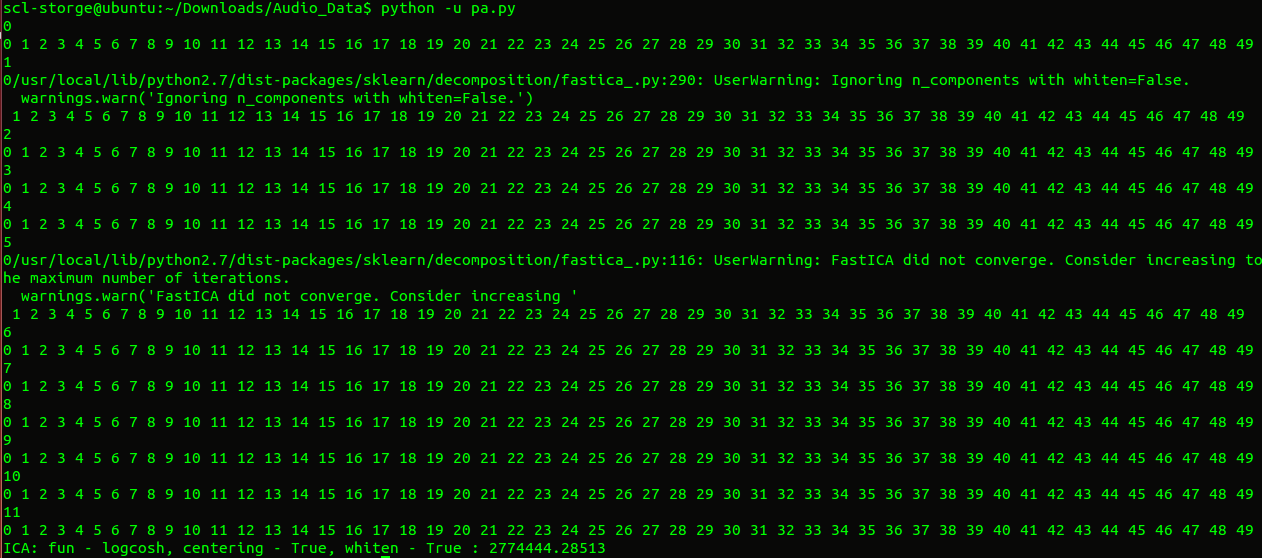
\includegraphics[width=\textwidth]{run}
	\caption{the best ICA is determined after 50 runs}
\end{figure}

\begin{figure}[H]
	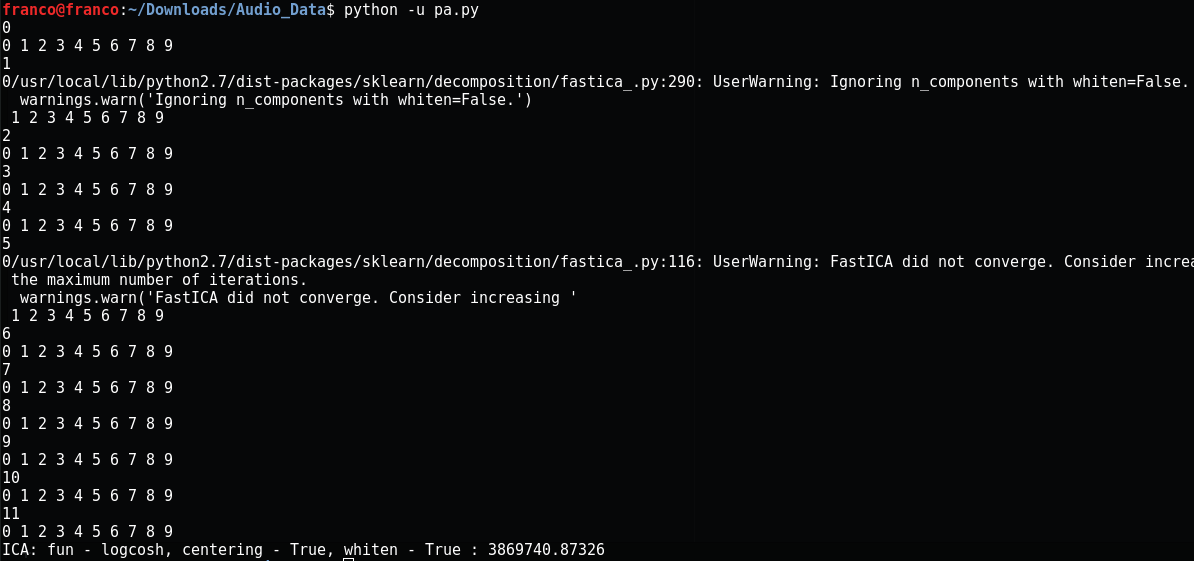
\includegraphics[width=\textwidth]{run2}
	\caption{the best ICA is determined after 10 runs}
\end{figure}

The FastICA algorithm might not converge to a solution given function $g_3$, centering disabled and whitening enabled. To get results with low residual, centering is required, whitening is necessary for preprocessing and the appropriate contrastive function is $g_1(y) = \frac{1}{a} \log \cosh (a * y)$. The residual values are also printed when the program is run. In general, whitening and centering is not necessary for FastICA, but may produce larger residual.

The independent files are now obtained including one with a male person speaking and the other is an orchestral music. The independent sounds are significantly lesser in volume than the signals from the original observations.

\begin{thebibliography}{9}

\bibitem{bib:sampling} P. Krishna, M. Rajasekhara, E. Ariwa, \emph{Global Trends in Information Systems and Software Applications, 4th ed.}, 2011

\end{thebibliography}

\end{document}